\documentclass[10pt]{beamer}
\usetheme[progressbar=frametitle]{metropolis}
% 'wolf' color theme replaced inline: that file isn't a standard Beamer package (it lived
% alongside the other project's main.tex) and Overleaf cannot find it. This reproduces its
% one visible effect here -- NC State red as the accent color -- without depending on the file.
\definecolor{ncred}{RGB}{204,0,0}
\setbeamercolor{frametitle}{bg=ncred, fg=white}
\setbeamercolor{progress bar}{fg=ncred, bg=ncred!20}
\setbeamercolor{title separator}{fg=ncred}
\setbeamercolor{alerted text}{fg=ncred}
\usepackage{appendixnumberbeamer}

\usepackage{booktabs}
\usepackage[scale=2]{ccicons}

\usepackage{pgfplots}
\usepgfplotslibrary{dateplot}

\usepackage{graphicx}    % for \includegraphics
\usepackage{subcaption}
\usepackage{colortbl}

\usepackage{xspace}
\newcommand{\themename}{\textbf{\textsc{metropolis}}\xspace}

\usepackage{tikz}
\usetikzlibrary{arrows.meta,decorations.pathreplacing,positioning}



\title{CircuitEvolve}
\subtitle{LLM-proposed circuit rewrites, decided by an exact verifier}
\author{Shubdeep Mohapatra}
\institute{North Carolina State University}
\titlegraphic{%
    \IfFileExists{ncstate_red_letter_logo.png}{\includegraphics[width=.5\textwidth]{ncstate_red_letter_logo.png}\hfill}{}
}

\makeatletter
\setbeamertemplate{title page}{
  \begin{minipage}[b][\paperheight]{\textwidth}
    \vfill%
    \ifx\inserttitle\@empty\else\usebeamertemplate*{title}\fi
    \ifx\insertsubtitle\@empty\else\usebeamertemplate*{subtitle}\fi
    \usebeamertemplate*{title separator}
    \ifx\beamer@shortauthor\@empty\else\usebeamertemplate*{author}\fi
    \ifx\insertdate\@empty\else\usebeamertemplate*{date}\fi
    \ifx\insertinstitute\@empty\else\usebeamertemplate*{institute}\fi
    \vfill
    \ifx\inserttitlegraphic\@empty\else\inserttitlegraphic\fi
    \vspace*{1cm}
  \end{minipage}
}
\makeatother

\begin{document}

\begin{frame}
    \titlepage
\end{frame}


\begin{frame}{One pipeline, one slot that changes}

\centering
\resizebox{0.85\textwidth}{!}{%
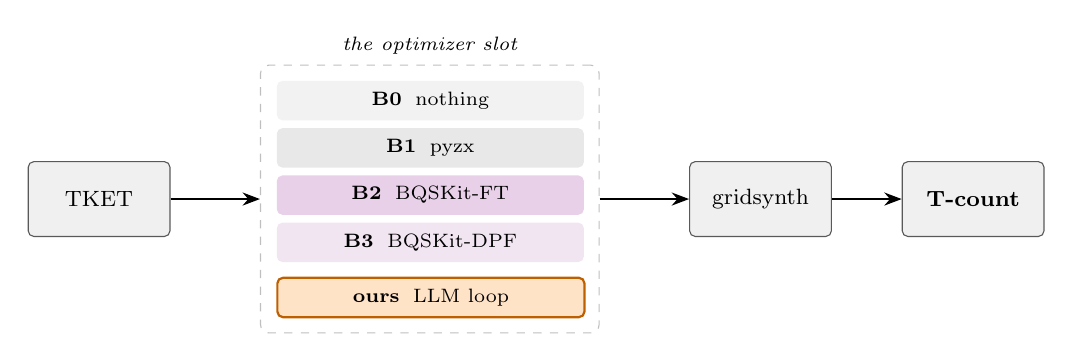
\begin{tikzpicture}[x=1cm, y=1cm,
    fix/.style={draw=gray!70!black, fill=gray!12, rounded corners=2pt, minimum width=1.8cm,
                minimum height=0.95cm, font=\footnotesize, align=center},
    slot/.style={draw=gray!50, dashed, rounded corners=3pt, minimum width=4.3cm, minimum height=3.4cm},
    opt/.style={rounded corners=2pt, minimum width=3.9cm, minimum height=0.5cm, font=\scriptsize,
                anchor=west, inner sep=3pt, align=left},
    arr/.style={-{Stealth[length=2.2mm]}, line width=0.8pt}]
  \node[fix] (T) at (0,0) {TKET};
  \node[slot] (S) at (4.2,0) {};
  \node[fix] (G) at (8.4,0) {gridsynth};
  \node[fix] (N) at (11.1,0) {\textbf{T-count}};
  \draw[arr] (T) -- (S); \draw[arr] (S) -- (G); \draw[arr] (G) -- (N);
  \node[font=\scriptsize\itshape] at (4.2,1.95) {the optimizer slot};
  \node[opt, fill=gray!10]            at (2.25, 1.25) {\textbf{B0}\; nothing};
  \node[opt, fill=gray!18]            at (2.25, 0.65) {\textbf{B1}\; pyzx};
  \node[opt, fill=violet!18]          at (2.25, 0.05) {\textbf{B2}\; BQSKit-FT};
  \node[opt, fill=violet!10]          at (2.25,-0.55) {\textbf{B3}\; BQSKit-DPF};
  \node[opt, fill=orange!22, draw=orange!75!black, line width=0.8pt] at (2.25,-1.25)
       {\textbf{ours}\; LLM loop};
\end{tikzpicture}%
}

\vspace{0.35cm}
\begin{itemize}
  \item Every bar in this talk is \textbf{T-count $\div$ B0} --- same circuit, same error budget, one slot swapped
\end{itemize}

\end{frame}


\begin{frame}{Inside our slot}

\centering
\resizebox{0.85\textwidth}{!}{%
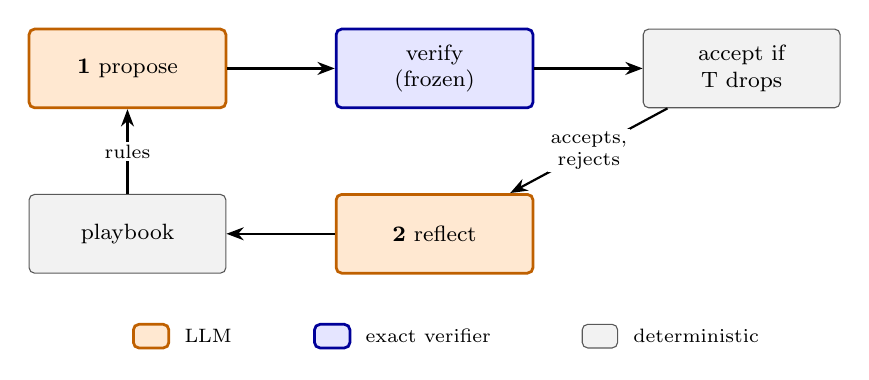
\begin{tikzpicture}[x=1cm, y=1cm,
    box/.style={draw=gray!70!black, fill=gray!10, rounded corners=2pt, minimum width=2.5cm,
                minimum height=1.0cm, font=\footnotesize, align=center},
    llm/.style={box, draw=orange!75!black, fill=orange!18, line width=1pt},
    ver/.style={box, draw=blue!60!black, fill=blue!10, line width=1pt},
    arr/.style={-{Stealth[length=2.2mm]}, line width=0.8pt},
    lab/.style={font=\scriptsize, midway, fill=white, inner sep=1pt, align=center}]
  \node[llm] (P) at (0,0)   {\textbf{1} propose};
  \node[ver] (V) at (3.9,0) {verify\\(frozen)};
  \node[box] (A) at (7.8,0) {accept if\\T drops};
  \node[llm] (R) at (3.9,-2.1) {\textbf{2} reflect};
  \node[box] (B) at (0,-2.1)  {playbook};
  \draw[arr] (P) -- (V); \draw[arr] (V) -- (A);
  \draw[arr] (A) -- node[lab]{accepts,\\rejects} (R);
  \draw[arr] (R) -- (B);
  \draw[arr] (B) -- node[lab]{rules} (P);
  \node[llm, minimum width=0.45cm, minimum height=0.3cm, font=\tiny] at (0.3,-3.4) {};
  \node[right, font=\scriptsize] at (0.6,-3.4) {LLM};
  \node[ver, minimum width=0.45cm, minimum height=0.3cm, font=\tiny] at (2.6,-3.4) {};
  \node[right, font=\scriptsize] at (2.9,-3.4) {exact verifier};
  \node[box, minimum width=0.45cm, minimum height=0.3cm, font=\tiny] at (6.0,-3.4) {};
  \node[right, font=\scriptsize] at (6.3,-3.4) {deterministic};
\end{tikzpicture}%
}

\vspace{0.2cm}
\begin{itemize}
  \item Two methods use this loop: \textbf{reconstruction} (Toffoli circuits) and \textbf{angle} (rotation circuits)
\end{itemize}

\end{frame}

\begin{frame}{Reconstruction: the LLM picks a compilation plan}

{\footnotesize\itshape What the prompt contains:}\\[1pt]
{\scriptsize Objective + contract (exact / relaxed) \textbullet\ Circuit summary, qubit roles \textbullet\ Recognized structure: Toffolis, pairs, multi-controlled cascades \textbullet\ Technique cards (toolbox) \textbullet\ Best verified so far + recent results \textbullet\ Playbook rules \textbullet\ Reply format: one JSON plan}

\vspace{0.2cm}
\colorbox{blue!7}{\parbox{0.97\linewidth}{\scriptsize \texttt{CIRCUIT barenco\_tof\_5: 9 qubits, 12 gates (ccx:12)}\\\texttt{PAIRS  P0 = T3+T9 (g3..g9) target q5 controls q0 q1: mirror}}}

\vspace{0.35cm}
\begin{center}
\colorbox{orange!16}{\parbox{2.8cm}{\centering\normalsize proposer LLM}}
\qquad$\Longrightarrow$\qquad
{\scriptsize\itshape returns a JSON plan}
\end{center}

\vspace{0.35cm}
\colorbox{blue!7}{\parbox{0.97\linewidth}{\scriptsize \texttt{\{"target": "relaxed", "decisions": [}\\\texttt{  \{"element": "M0", "route": "ancilla\_mcx", "middle": "jones"\},}}}

\vspace{0.25cm}
\raggedright\footnotesize
A deterministic compiler executes the plan; the frozen verifier accepted it: $84 \to 36$ T (barenco\_tof\_5, call 1).

\end{frame}

\begin{frame}{Angle: the LLM rewrites one window}

{\footnotesize\itshape What the prompt contains:}\\[1pt]
{\scriptsize Task + gate set \textbullet\ Cost model (gridsynth T per rotation) \textbullet\ Error allowance for this window \textbullet\ Two actions: rewrite window or fix rotations \textbullet\ The window itself (at most 4 qubits, 40 gates) \textbullet\ Playbook rules \textbullet\ Recent verifier feedback}

\vspace{0.2cm}
\colorbox{blue!7}{\parbox{0.97\linewidth}{\scriptsize \texttt{rz at a multiple of pi/4 is exact; every other rz costs \textasciitilde{}46 T}\\\texttt{allowance = 6.250e-05 (phase-aligned operator-norm distance)}}}

\vspace{0.35cm}
\begin{center}
\colorbox{orange!16}{\parbox{2.8cm}{\centering\normalsize proposer LLM}}
\qquad$\Longrightarrow$\qquad
{\scriptsize\itshape returns replacement gates}
\end{center}

\vspace{0.35cm}
\colorbox{blue!7}{\parbox{0.97\linewidth}{\scriptsize \texttt{op 9 rz(+pi/8) and op 17 t q1 share Pauli frame +IZII}\\\texttt{-> exact merge, angle 0.3927 + pi/4 = 3pi/8}}}

\vspace{0.25cm}
\raggedright\footnotesize
Verifier accepted the two frame merges: $2115 \to 2114$ T (qft\_8, call 2). Parsed by regex --- never executed.

\end{frame}

\begin{frame}{Every 8 calls: the reflector edits the playbook}

{\footnotesize\itshape What the prompt contains:}\\[1pt]
{\scriptsize Current playbook with A/B statistics \textbullet\ Accepted improvements (parent to child) \textbullet\ Recent rejections and the exact verifier reason \textbullet\ Reply: at most 3 add / edit / retire}

\vspace{0.2cm}
\colorbox{blue!7}{\parbox{0.97\linewidth}{\scriptsize \texttt{R18 [candidate; shown 20; improving w/ 0/20, w/o 0/19]}\\\texttt{rejected: op 24->0: distance 2.330e-04 > allowance 6.250e-05}}}

\vspace{0.35cm}
\begin{center}
\colorbox{orange!16}{\parbox{2.8cm}{\centering\normalsize reflector LLM}}
\qquad$\Longrightarrow$\qquad
{\scriptsize\itshape returns rule edits}
\end{center}

\vspace{0.35cm}
\colorbox{blue!7}{\parbox{0.97\linewidth}{\scriptsize \texttt{\{"op": "edit", "id": "R18", "text": "..."\}}\\\texttt{\{"op": "retire", "id": "R17", "why": "..."\}}}}

\vspace{0.25cm}
\raggedright\footnotesize
New rules enter as CANDIDATES and are shown to half the prompts; only measured T reduction promotes them.

\end{frame}


% =====================================================================
\section{Results}
% =====================================================================

\begin{frame}{Reconstruction, trained circuits}

\centering
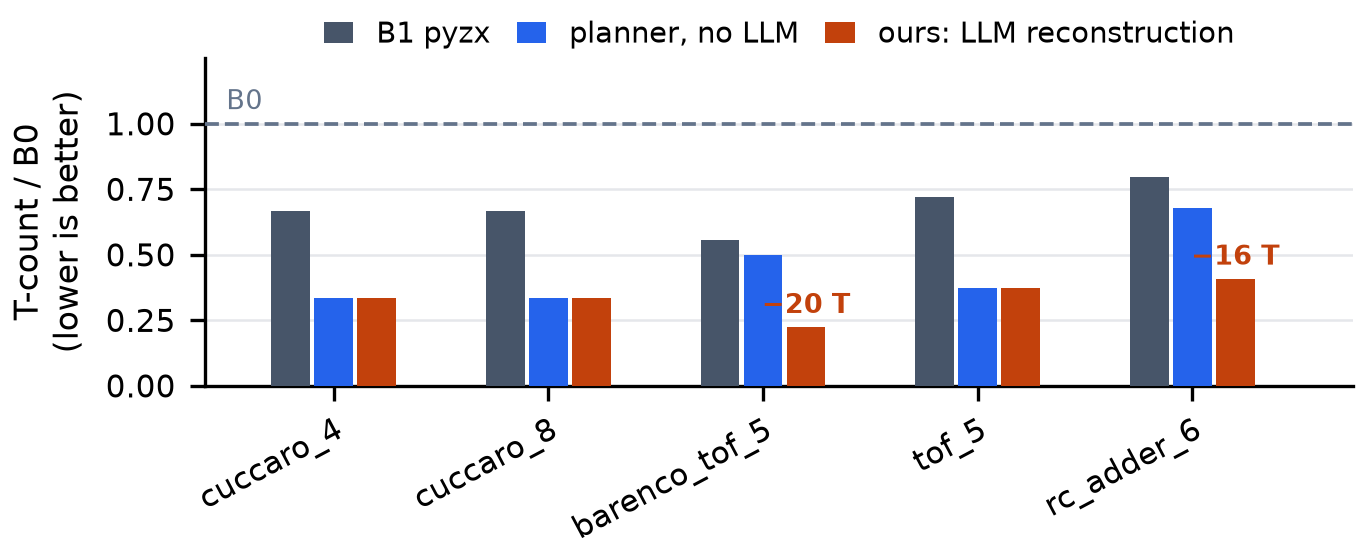
\includegraphics[width=0.96\textwidth]{circuitevolve_figs/fig_recon_trained.png}

\begin{itemize}
  \item Beats pyzx on 5 of 5; largest gain on cuccaro\_8, $-32$ T
\end{itemize}
\vspace{-0.05cm}
\raggedright\scriptsize
Ours uses the relaxed contract (ancillas + measurement, every branch verified exactly); B0, B1 are exact. These circuits carry no continuous rotations, so gridsynth is a no-op.

\end{frame}


\begin{frame}{Reconstruction, circuits it never saw}

\centering
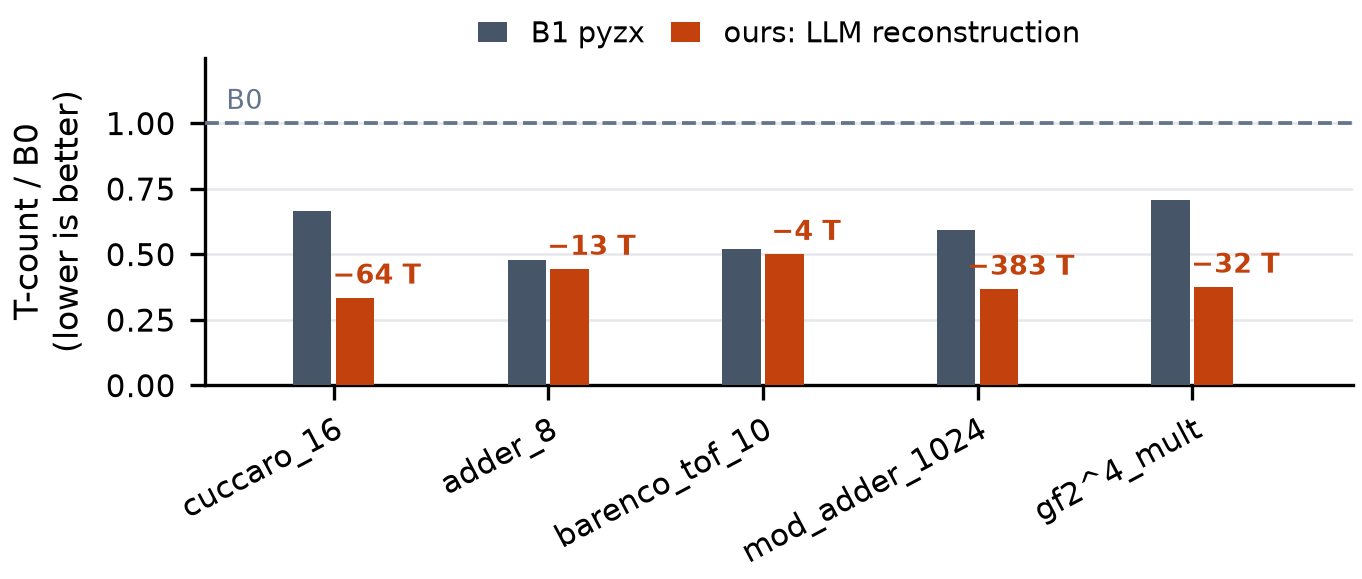
\includegraphics[width=0.96\textwidth]{circuitevolve_figs/fig_recon_frozen.png}

\begin{itemize}
  \item Playbook frozen, reflector off --- beats pyzx on all 5, up to $-383$ T on mod\_adder\_1024
\end{itemize}
\vspace{-0.05cm}
\raggedright\scriptsize
Four further frozen circuits have no B0/B1 reference: ham15-med $-5\%$, gf2$^6$\_mult $0\%$, hwb6 $-7\%$, mod\_red\_21 $-21\%$ vs the deterministic control route.

\end{frame}


\begin{frame}{Angle: our approach barely moves}

\centering
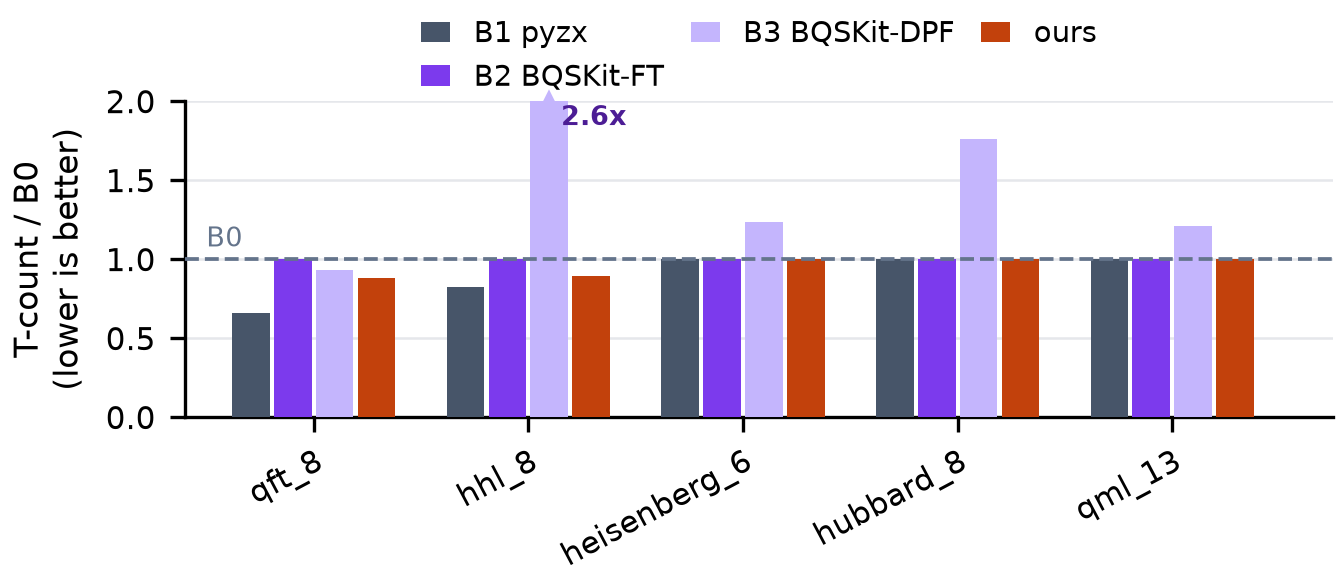
\includegraphics[width=0.96\textwidth]{circuitevolve_figs/fig_angle.png}

\begin{itemize}
  \item B2 lands exactly on B0; B3 is worse than B0 on 4 of 5
  \item Ours is close to B0 everywhere --- a deterministic merge pass does almost all of it, the LLM adds $\leq 0.5\%$ on top
\end{itemize}
\vspace{-0.05cm}
\raggedright\scriptsize
A supplementary DPF variant does better than all of these on hhl\_8 ($0.55\times$ B0); appendix table.

\end{frame}


\begin{frame}{Where the two stages compose}

\centering
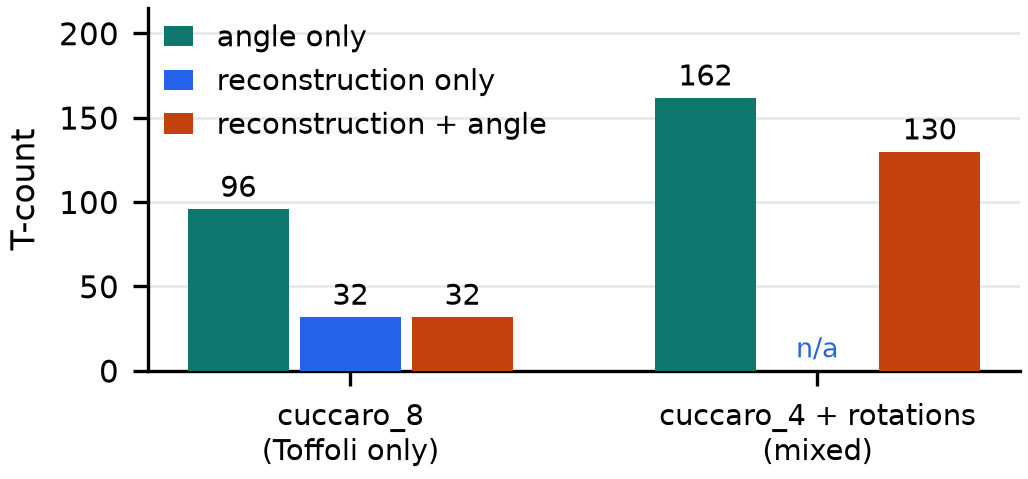
\includegraphics[width=0.72\textwidth]{circuitevolve_figs/fig_stages.png}

\begin{itemize}
  \item Reconstruction does the work; the angle stage adds nothing after it
\end{itemize}
\vspace{-0.05cm}
\raggedright\scriptsize
Zero-LLM demo (deterministic planner + merge pass). Reconstruction alone is not defined on the mixed circuit: it leaves the rotations untouched. An LLM cascade run is still to do.

\end{frame}


\begin{frame}{Reconstruction learned rules; angle did not}

\centering
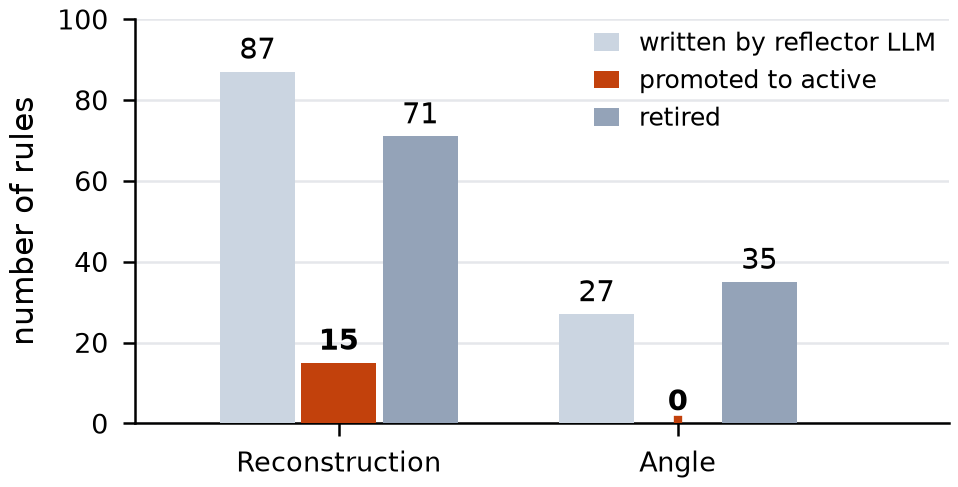
\includegraphics[width=0.74\textwidth]{circuitevolve_figs/bar_rules.png}

\begin{itemize}
  \item 15 rules promoted by the A/B test, then used frozen on unseen circuits
  \item Angle: 0 promoted --- playbook, placebo and no-playbook arms end at the same T
\end{itemize}

\end{frame}


\begin{frame}{Conclusions}

\begin{itemize}
  \setlength\itemsep{10pt}
  \item Reconstruction: beats the deterministic planner on \textbf{8 of 14} circuits, \textbf{6 of 9} never trained on
  \item One discovery became \textbf{exact code} and now runs with zero LLM calls
  \item Angle windows: no headroom after TKET; the remaining gains are global, not local
  \item Next: let the LLM propose \textbf{passes}, not windows
\end{itemize}

\end{frame}


\appendix

\begin{frame}{Appendix: reconstruction, T-count}

\centering
\scriptsize
\renewcommand{\arraystretch}{1.05}
\begin{tabular}{>{\centering}m{2.3cm} >{\centering}m{1.5cm} >{\centering}m{1.2cm} >{\centering}m{1.2cm} >{\centering}m{1.3cm} >{\centering\arraybackslash}m{1.2cm}}
  \rowcolor{ncred}
  \color{white}\textbf{Circuit} & \color{white}\textbf{split} & \color{white}\textbf{B0} & \color{white}\textbf{B1} & \color{white}\textbf{planner} & \color{white}\textbf{ours} \\
  \rowcolor{lightgray}
  cuccaro\_4 & dev & 48 & 32 & 16 & 16 \\
  cuccaro\_8 & dev & 96 & 64 & 32 & 32 \\
  \rowcolor{lightgray}
  barenco\_tof\_5 & dev & 72 & 40 & 36 & \textbf{16} \\
  tof\_5 & dev & 43 & 31 & 16 & 16 \\
  \rowcolor{lightgray}
  rc\_adder\_6 & dev & 59 & 47 & 40 & \textbf{24} \\
  cuccaro\_16 & held-out & 192 & 128 & 64 & 64 \\
  \rowcolor{lightgray}
  adder\_8 & held-out & 361 & 173 & 180 & \textbf{160} \\
  barenco\_tof\_10 & held-out & 192 & 100 & 96 & 96 \\
  \rowcolor{lightgray}
  mod\_adder\_1024 & held-out & 1711 & 1011 & 660 & \textbf{628} \\
  gf2$^4$\_mult & held-out & 96 & 68 & 64 & \textbf{36} \\
  \rowcolor{lightgray}
  ham15-med & reserved & -- & -- & 220 & \textbf{208} \\
  gf2$^6$\_mult & reserved & -- & -- & 144 & 144 \\
  \rowcolor{lightgray}
  hwb6 & reserved & -- & -- & 56 & \textbf{52} \\
  mod\_red\_21 & reserved & -- & -- & 56 & \textbf{44} \\
\end{tabular}

\vspace{0.1cm}
\raggedright\tiny
Bold: below the planner. B0 = TKET, B1 = pyzx (both exact); planner and ours relaxed. $\mathrm{--}$: not computed.

\end{frame}


\begin{frame}{Appendix: angle, T-count at $\varepsilon = 10^{-3}$}

\centering
\scriptsize
\renewcommand{\arraystretch}{1.1}
\begin{tabular}{>{\centering}m{2.0cm} >{\centering}m{1.1cm} >{\centering}m{1.1cm} >{\centering}m{1.1cm} >{\centering}m{1.1cm} >{\centering}m{1.25cm} >{\centering}m{1.3cm} >{\centering\arraybackslash}m{1.1cm}}
  \rowcolor{ncred}
  \color{white}\textbf{Circuit} & \color{white}\textbf{B0} & \color{white}\textbf{B1} & \color{white}\textbf{B2} & \color{white}\textbf{B3} & \color{white}\textbf{B3 (var.)} & \color{white}\textbf{merge pass} & \color{white}\textbf{+ LLM} \\
  \rowcolor{lightgray}
  qft\_8 & 2391 & 1577 & 2391 & 2226 & 2029 & 2115 & 2113 \\
  heisenberg\_6 & 8200 & 8200 & 8200 & 10128 & 8600 & 8200 & 8200 \\
  \rowcolor{lightgray}
  hubbard\_8 & 4312 & 4312 & 4312 & 7588 & 4712 & 4312 & 4312 \\
  qml\_13 & 6326 & 6326 & 6326 & 7668 & 6790 & 6326 & 6326 \\
  \rowcolor{lightgray}
  hhl\_8 & 35450 & 29205 & 35450 & 93637 & 19443 & 31762 & 31615 \\
  qpe\_8 & 14761 & 11485 & 14761 & 39565 & 8020 & 12597 & -- \\
  \rowcolor{lightgray}
  qae\_13 & 7821 & 4527 & 7821 & 7516 & 6909 & 6683 & -- \\
  tfim\_6 & 8560 & 8560 & 8560 & 12990 & 9600 & 8560 & -- \\
\end{tabular}

\vspace{0.1cm}
\raggedright\tiny
B3 (var.) = supplementary DPF + gridsynth variant. Last two columns: our slot without and with the LLM. Blank = not run (campaign paused).

\end{frame}


\end{document}
